\begin{proof}
    We have to use \textbf{averaged} uniform stab (this is a randomized algo!).
    
    Notation shortcuts : \begin{itemize}
        \item A($\mathcal{D}_n$, t steps) $\equiv \theta_t$
        \item A($\mathcal{D}_n^{(k)}$, t steps) $\equiv \tilde{\theta_t}$
    \end{itemize}
    
    $\forall t \geq 1$,
    \begin{align*}
        \mathbb{E} 
            & [ \left\| \theta_{t+1} - \tilde{\theta_{t+1}} \right\| | \mathcal{F}_t ]
            & = \mathbb{E}[ \left\| \theta_{t+1} - \tilde{\theta_{t+1}} \right\| \mathbbm{1}_{i(t+1)= k} + \left\| \theta_{t+1} - \tilde{\theta_{t+1}} \right\| \mathbbm{1}_{i(t+1)\neq  k}| \mathcal{F}_t] \\
            & = \frac{1}{n} \mathbb{E}[ \left\| \theta_{t+1} - \tilde{\theta_{t+1}} \right\| | \mathcal{F}_t, i(t+1)= k] + \frac{n-1}{n} \mathbb{E}[ \left\| \theta_{t+1} - \tilde{\theta_{t+1}} \right\| | \mathcal{F}_t, i(t+1) \neq k]
    \end{align*}
    
    \begin{itemize}
        \item Conditionally to $i(t+1) = k$ ($\mathbb{E}[ \left\| \theta_{t+1} - \tilde{\theta_{t+1}} \right\| | \mathcal{F}_t, i(t+1)= k]$) , 
        \[
            \left\| \theta_{t+1} - \tilde{\theta_{t+1}} \right\| \leq \left\| \theta_{t} - \tilde{\theta_{t}} \right\| + \gamma _t ( \left\| \nabla \psi_k (\theta _k) \right\| + \left\| \nabla \tilde{\psi_k} (\tilde{\theta _k}) \right\|)
        .\]
        $\left\| \nabla \psi_k (\theta _k) \right\| \leq BR$ \\
        $\left\| \nabla \tilde{\psi_k} (\tilde{\theta _k}) \right\| \leq BR$

        \item Conditionally to $i(t+1) \neq  k$, the non-expensivness property gives that $\left\|  \theta_{t+1} - \tilde{\theta_{t+1}} \right\| \leq \left\|  \theta_{t} - \tilde{\theta_{t}} \right\|$ \\
        Therefore,
        
        \begin{align*}
            \mathbb{E}[ \left\| \tilde{\theta_{t+1}} - \theta_{t+1} \right\| | \mathcal{F}_t] &\leq \frac{1}{n} \left\| \theta_{t} - \tilde{\theta_{t}} \right\| + \frac{n-1}{n} \left\| \theta_{t} - \tilde{\theta_{t}} \right\| \\
            & = \left\| \theta_{t} - \tilde{\theta_{t}} \right\| + \frac{\gamma _ {t+1} 2BR}{n} \\
            & \dots \\
            & \leq \left\| \theta_0 - \tilde{\theta _0} \right\|  + \frac{\sum_{u=1}^{t+1}}{n}
        \end{align*}

        As previously, we have obtained a bound on $\left\| A(\mathcal{D}_n, T steps) - A(\mathcal{D_n^{(k)}}, T steps) \right\| $ witch leads to uniform stability with $\beta (n) = \frac{2B^2R^2 \sum_{t=1}^{T}\gamma _t}{n}$
    \end{itemize}
\end{proof}
        
\textbf{Conclusion} What can be said about the generalization of SGD after T steps?
\begin{itemize}
    \item Recall that for $T \leq n$, without replacement (one pass over the data), we actually minimize the generalization risk directly : we already obtained a rate in the previous lecture. 
    \item For $ T \geq n $ (multipasses over the data) with rempalcement, Lemma 1 of this lecture give 
    \begin{align*}
        \mathcal{R}(A(\mathcal{D}_n, T)) - \mathcal{R}^\star 
        &\leq \underbrace{\beta (n,T)}_{\text{stability}} + \underbrace{Optim(T \text{ iter})}_{Optimisation} \\
        &\leq \underbrace{\frac{2 \beta ^2 R^2}{n }\sum_{}^{}\gamma _t}_{\text{Today}} + \underbrace{\frac{\left\| \theta _0 - \theta ^\star  \right\| }{\gamma T } + \gamma \sigma ^2}_{\text{with } \gamma \text{ cst (cf previus lecture)} }
    \end{align*}
\end{itemize}
\textbf{Good}: We have obtained a generalization bound for nay nb $ T $ of iteration \\
\textbf{Trade-off} between stability and optimisation. This suggest the existence of an optimal "EARLY STOPPING" time $ T^\star  $, such that the risk decreases up to $ T^\star  $     
\begin{figure}[!h]
    \centering
    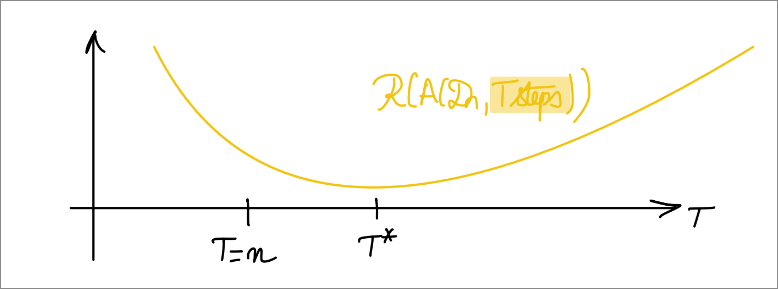
\includegraphics[width=.75\textwidth]{figs/early_stoping.png}
    \caption{Early Stopping : $ \min _\gamma \frac{C_1 T \gamma }{n } + \frac{C_2}{\gamma T} + \gamma \sigma ^2 \Rightarrow \gamma = \sqrt{\frac{C_2}{T(\frac{C_1 T}{n} + \sigma ^2)}} $ }
\end{figure}